\chapter{Detection Tools}
\section{Rule based Signature Detection}
A strategy to generalize the notion of signature is the matching of a \textit{set of
\textbf{rules}}:
A set of rules is more absract than a regular expression or a string, and such generalization can tolerate some changes in the body of the malware.

\textbf{Yara} rules are becoming the de facto standard for pattern matching,
which can be applied in many contexts,
including IDS rules but not only;
it has been made to discover and identify malware samples.

A well-known rule based detection tool is \textbf{Snort} IDS\footnote{\textit{Intrusion Detection System}}:
\begin{enumerate}
   \item A good \textbf{sniffer}
   \item A \textbf{rule} based detection engine
   \item Packets that do not match rules are neglected (by the analysis)
   \item Packet that match rules are analyzed and can even fire an advice
\end{enumerate}

\section{Yara}
Yara is quite simple:
\begin{enumerate}
   \item Open a text editor
   \item Write rules in Yara syntax
   \item Give Yara a set of files to be analyze
   \item Let Yara find evil for you
\end{enumerate}

A tool to identify and classify malware samples by creating descriptions of malware families based on textual or binary patterns.

An example of a Yara rule is provided below:
\begin{lstlisting}
   rule silent_banker : banker
   {  meta:
         description = "This is just an example"
         threat_level = 3
         In_the_wild = true
      strings:
         $a = {6A 40 68 00 30 00 00 6A 14 8D 91}
         $b = {8D 4D B0 2B C1 83 C0 27 99 6A 4E 59    F7 F9}
         $c = "UVODFRYSIHLNWPEJXQZAKCBGMT"
      condition:
         $a or $b or $c
   }
\end{lstlisting}

In this example any file/memory area containing one of the three \texttt{strings} must be reported as \texttt{silent\_banker}.

\subsubsection{Cuckoo Module}
There are also Yara modules used to introduce other features aside from Yara's native ones.

A relevant example is the \texttt{Cuckoo} module which allows to run a piece of code, capture some information about the behaviour
of the code and pass it to Yara,
making the performed analysis dynamic.

\begin{lstlisting}
   import "cuckoo"
   rule evil_doer 
   {
      string os:
         $some_string = { 01 02 03 00 05 06 } 

      condition:
         $some string and 
         cuckoo.netuork.http request(/http: vvsomeooe,eoioge 1 cam') 
    }
\end{lstlisting}

\section{Snort}
Snort, based on \texttt{libpcap}, provides three possible modes to operate in:
\begin{enumerate}
   \item \textbf{Sniffer}
   To output data in transit and also check the IP and TCP/ICMP/UDP headers:
   \lstinline|./snort -vd|
   \item \textbf{Logging}
   In case wanto to designate a logging directory \lstinline|. ./snort -vd|
   \item \textbf{NIDS}\footnote{\textit{\textbf{Network} Intrusion Detection System}}:
   NIDS mode allows to define through rules the action to take upon detection of
   malicious data packets.
\end{enumerate}

\begin{figure}[htbp]
   \centering
   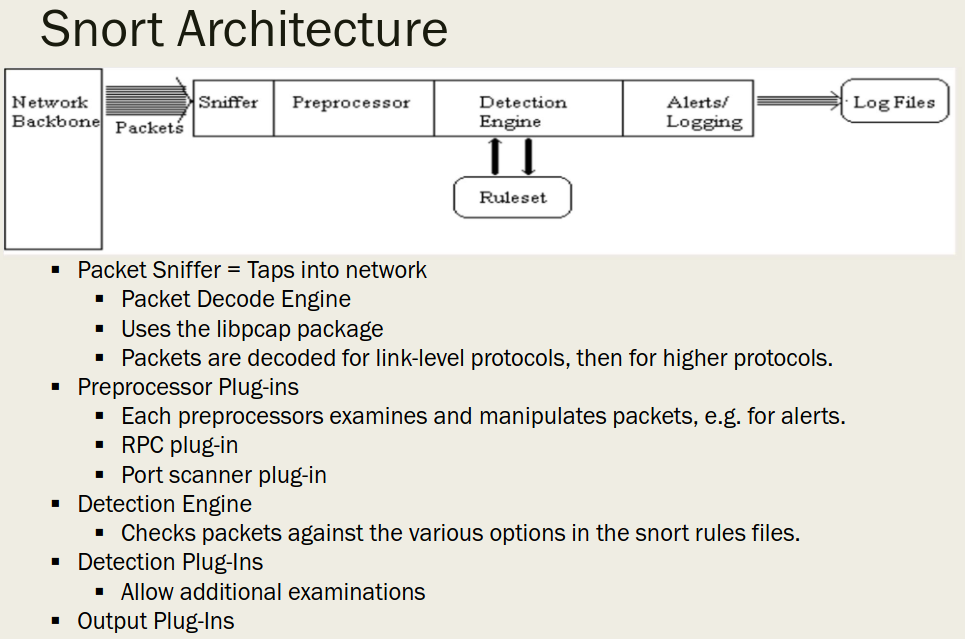
\includegraphics{images/snort_architecture.png}
   \caption{Snort architecture}
   \label{fig:snort_architecture}
\end{figure}

\newpage
\subsection*{Port Scanning - plugin}
Two common practices made by attackers to scan a network are port scanning, sweeping and walking.
There is a dedicated snort plugin to detect such actions. 
\begin{figure}[htbp]
   \centering
   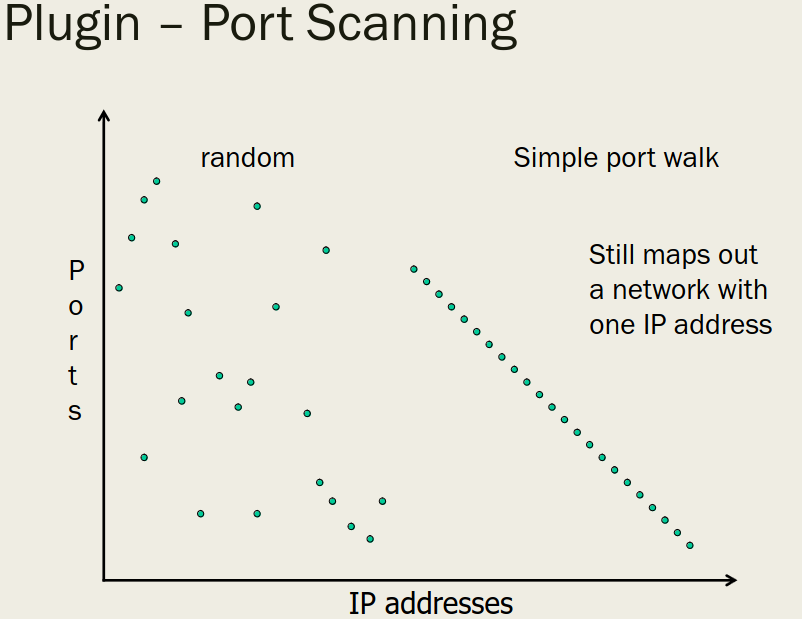
\includegraphics[width=0.45\columnwidth]{images/snort_port_1.png}
   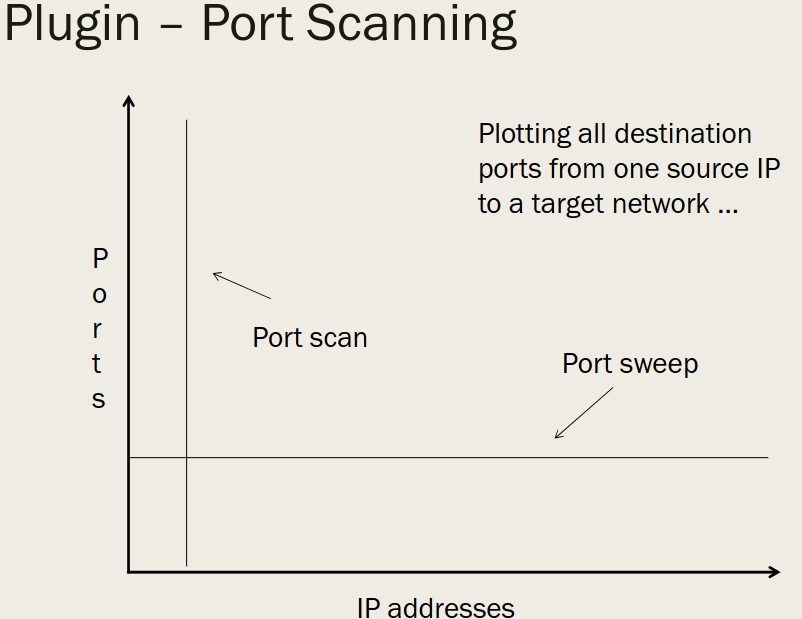
\includegraphics[width=0.45\columnwidth]{images/snort_port_2.png}
   \caption{Snort port scanning plugin}
   \label{fig:snort_port}
\end{figure}

\subsection{Rules}
\labelitemize{
   \textit{Snort rules structure}
}{
   \begin{enumerate}
      \item \textbf{Rule header}
      \begin{enumerate}
         \item The rule action,
         \item The protocol
         \item The source and destination IP addresses
         \item Network mask
         \item Information on source and destination port
      \end{enumerate}
      \item \textbf{Options section}
      \begin{enumerate}
         \item Messages
         \item Information on the packet sections to be examined to discover if the rule
         should be fired.
      \end{enumerate}
   \end{enumerate}
}

\begin{lstlisting}
   alert tcp any any -> any any (msg:"Possible Zeus Botnet C&C Traffic"; flow:established,to_server; content:"|5a 4f 4f 4d 00 00|"; depth:6; sid:1000005; rev:1;)
\end{lstlisting}

\labelitemize{
   \textit{Snort predefined \textbf{actions}}
}{
   \begin{enumerate}   
   \item \texttt{alert}: raise an alert and log the packet
   \item \texttt{log}: log the packet
   \item \texttt{pass}: neglect the packet
   \item \texttt{activate}: raise an alert and activate a dynamic rule (remember a state)
   \item \texttt{dynamic}: idle till it is activated then logs the packets
   \item \texttt{drop}: log and block the packet (not only a sniffer but also a filter)
   \item \texttt{reject}: block and log the packet and then send
   \begin{enumerate}
      \item TCP reset if TCP
      \item ICMP port unreacheable if UDP
   \end{enumerate}
   \item \texttt{sdrop}: block the packet but do not log it
   \end{enumerate}
}

Multiple rules might match a packet,
thus an order must be established.
The safest way is to apply rules in the order
\begin{center}
   \texttt{Drop > Pass > Alert > Log}
\end{center}
This order is safe yet very expensive in terms of computational resources and time,
since the \texttt{DROP} check \textit{overhead} is computed even for legal packets.
Since, most packets are legal and not dangerous,
a more effective but more dangerous option is
\begin{center}
   \texttt{Pass > Drop > Alert > Log}
\end{center}

\section{Merging Signatures and Anomalies}
\subsection{Endpoint Detection and Response}
An \textbf{EDR} or an \textit{endpoint threat detection and response} (\texttt{ETDR}) is an endpoint
security solution that merges monitoring and collecting information in
real time:
\textit{Real-time} \textbf{collected} information is analized and proper responses are fired by a \textbf{rule}-based system.

\textbf{EDR/ETDR} is used to describe systems currently developed that automate
the analysis of information and the responses to detected intrusions.

The \textbf{main tasks} of an ETDR include:
\begin{itemize}
   \item \textit{Endpoint monitoring} to collect information about possible intrusions
   \item \textit{Analyze and correlate} collected information to discover ongoing intrusions
   \item \textit{Automatic response} to intrusion to minimize the impacts
   \item Apply forensics tool to discover intrusions 
   \note{(even old ones)}
\end{itemize}

\begin{figure}[htbp]
   \centering
   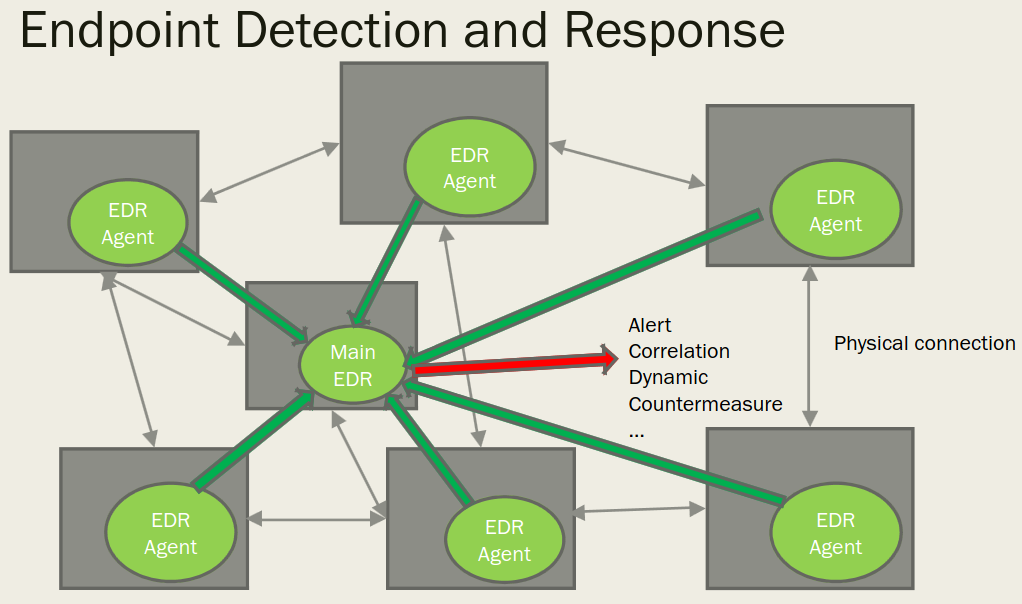
\includegraphics{images/EDTR_architecture.png}
   \caption{EDTR architecture}
   \label{fig:EDTR_architecture}
\end{figure}
\labelitemize{
   \textit{Main Components}
}{
   \begin{itemize}
      \item \textbf{Endpoint data collection agents}:
      collects information on security status and transmits it to a data \textit{collection
   center}.
      \note{It can also log information, apply patches, activate or kill processes.}
      It may analyze the memory, the files or the packets flowing across the node or
      implement anomaly detection.

      \item \textbf{Centralized analytical engine}. 
      It looks for patterns in the \textit{real-time data} and signals if an intrusion involves one or
      several nodes.
      It also coordinates the actions of the various agents.
      \note{
         It may use IOC, signature etc.
      }
      \item \textbf{Forensics analysis}:
      An EDR may implenent forensic analysis to discover  intrusion that have exploited new vulnerabilities and new attack techniques.
      The forensics component may discover old undetected intrusions to produce data
      on still unknown techniques.
      This analysis does not need to be run in real time.
   \end{itemize}
}

Looks like gold, but in fact, there is \textbf{not} much \textbf{correlation} happening in the central node,
and EDR agents are not so powerful defenders,
even if more advanced than legacy antiviruses,
since they monitor the ongoing operation, scan images as they are
run or the node memory, covering a much larger number of
attacks.

The main \textbf{goal} of \textbf{EDR} is \textit{automating} the work of a defender.
This reduces the investment in cyber security and enables an
organization to \textit{monitor} its infrastructure.

\subsection{Introspection}
A mechanism which resides in the EDR family, is \textbf{Virtual Machine Introspection} which formally defines techniques and tools to monitor a VM run time behavior to protect a VM from internal and external attacks

\labelitemize{
   \textit{Key-Points}
}{
   \begin{itemize}
      \item 
      Along with introspection some basic security mechanism are provided, such as
      \textit{virus scanners} and \textit{IDS}s.
      \item 
      Observe and respond to VM events from a \textit{"safe"} location \textit{outside} the
      monitored machine.
      \item Exploit virtualization as a countermeasure. 
      It is an example of how
      virtualization changes the computing framework.
      \item With respect to static attestation, VMI implements a
      form of run time attestation that aims to discover not only which software a
      system runs but also its run time integrity.
   \end{itemize}
}

\begin{figure}[htbp]
   \centering
   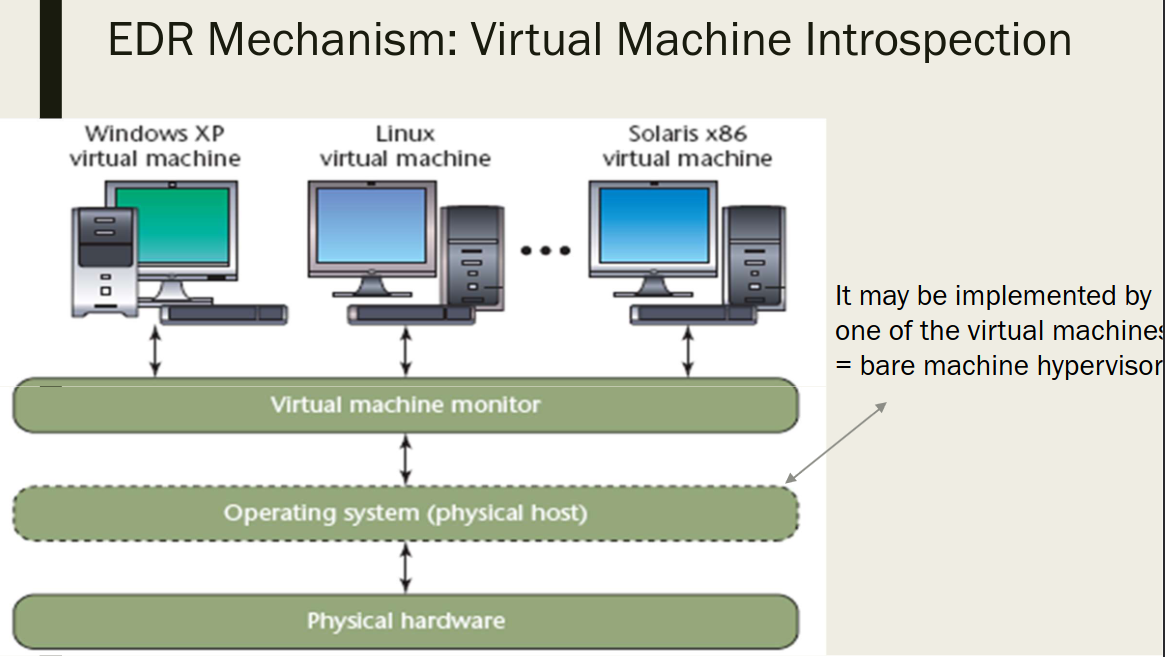
\includegraphics{images/VMI_arch.png}
   \caption{VMI arch}
   \label{fig:VMI_arch}
\end{figure}

VMI defines a \textbf{Memory Mapping} system\footnote{Actually it is not clear from the slides where does this Memory mapping comes out} to seamlessly and easily manage memory accesses,
through advanced memory translation.

Besides there is a mechanism to check the integrity of virtual components,
based on a chain of trust,
which is both a strength and a possible point-of-failure.

\begin{figure}[htbp]
   \centering
   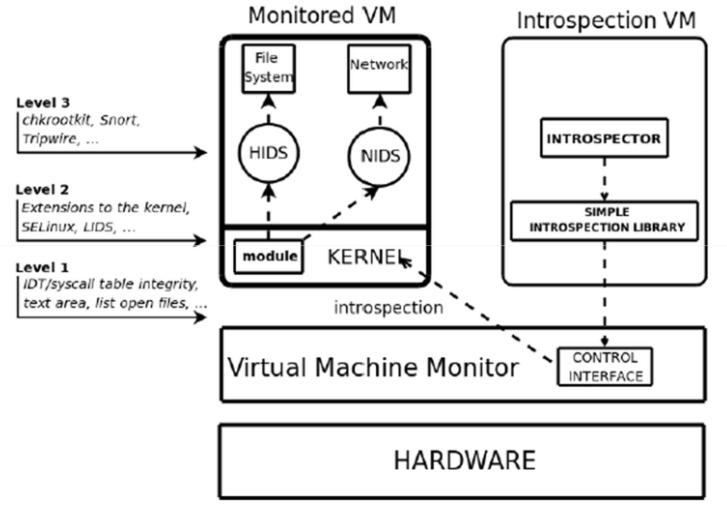
\includegraphics{images/VMI_trustchain.png}
   \caption{VMI Chain of Trust}
   \label{fig:VMI_trustchain.png}
\end{figure}